\documentclass[12pt]{article}

\usepackage[T1,T2A]{fontenc}
\usepackage[english]{babel}
\usepackage[type1]{libertine}
\usepackage{microtype}

\babelprovide[import,main]{serbian-cyrillic}

\newcommand\textenglish[1]%
{\foreignlanguage{english}{\fontencoding{T1}\selectfont#1}}
\newenvironment{english}%
{\begin{otherlanguage}{english}\fontencoding{T1}\selectfont}%
	{\end{otherlanguage}}

\NeedsTeXFormat{LaTeX2e}[1994/06/01]
\ProvidesPackage{pek}

\RequirePackage{amsmath, amsfonts, amssymb, amsthm, braket, bbold, fullpage, tikz, pgfplots, pgffor, empheq, mathtools}
\usetikzlibrary {positioning}
\newcommand{\crtNaH}[1]{\draw (#1,-0.1) node[anchor=north] {#1}  [thick] (#1, -0.1) -- (#1, 0.1);}
\newcommand{\bd}{\textbf}
\newcommand{\evl}[3]{|_{#1=#2}^{#1=#3}}


\newcommand{\graf}[7]{
	
	\begin{scope}
		\clip (-0.1,-0.1) rectangle (#1,#3);
		\draw[->] (-0.1,0) -- (#1,0) node[below] {$#2$};
		\draw[->] (0,-0.1) -- (0,#3) node[left] {$#4$};
		
		
		\clip (0,0) rectangle (#1,#3);
		\draw[scale=1,domain=0:#7,smooth,variable=#5,black] plot ({#5}, {#6});
	\end{scope}

	\foreach \n in {1,...,#1}{
		\draw (\n,-0.1) node[anchor=north] {\n}  [thick] (\n-1, -0.1) -- (\n-1, 0.1);
	}

	\foreach \n in {1,...,#3}{
			\draw (-0.1,\n) node[anchor=east] {\n}  [thick] (-0.1, \n-1) -- (0.1, \n-1);
	}
	

	\draw (0,-0.09) node[anchor=north] {0};
}


\endinput
\usepackage{graphicx}
\usepackage{subcaption}
\usepackage{float}
\usepackage[export]{adjustbox}

\usepackage{listings}
\usepackage{color}


\definecolor{dkgreen}{rgb}{0,0.6,0}
\definecolor{gray}{rgb}{0.5,0.5,0.5}
\definecolor{mauve}{rgb}{0.58,0,0.82}

\lstset{frame=tb,
	language=c++,
	aboveskip=3mm,
	belowskip=3mm,
	showstringspaces=false,
	columns=flexible,
	basicstyle={\small\ttfamily},
	numbers=none,
	numberstyle=\tiny\color{gray},
	keywordstyle=\color{blue},
	commentstyle=\color{dkgreen},
	stringstyle=\color{mauve},
	breaklines=true,
	breakatwhitespace=true,
	tabsize=3
}


\title{Рендеровање}
\author{Теодор Ђелић}
\date{Јун 2020}



\begin{document}
	
	\maketitle
	
	\section*{Апстракт}
	У овом раду ћете сазнати шта је компјутерска графика, шта је рендеровање, историјат његовог развоја, , као и различите технике његове реализације. Приказаћемо илустрацију рендеровања кроз пример-апликацију која користи модерну имплементацију OpenGL-а.
	
	\section{Увод}
	
	\subsection{Компјутерска графика}
	\paragraph{}
	Компјутерска графика је једна од подобласти компјутерских наука која се, најпростије речено, бави свим процесима који су везани за приказивање слике на екрану, односно од самог процеса обликовања и стварања података који чувају информације облика и модела за приказ, обраде тих информација и текстура, рендеровање и осветљавање модела, све до дигиталних приказа слика на екрану.
	\subsection{Рендеровање као појам}
	\paragraph{}
	Као што смо споменули, рендеровање је кључан део у процесу приказивања слике на екрану. Описали бисмо рендеровање као процес генерисања слике из неких података помоћу софтверског програма. Наравно, овај опис је апстрактан (знамо и сами да се процес генерисања слике у фотошопу разликује од процеса цртања појединачних фрејмова у игрици), па зато и делимо рендеровање по различитим критеријумима на више подгрупа. За критеријум можемо узети разне факторе (нпр. да ли је жељена фотореалистична слика или не), али постоји један који је изнад свих, односно он је онај примарни те га узимамо за главну поделу, а то је критеријум важности брзине извршавања и по њему делимо рендеровање у две категорије: рендеровање у реалном времену и споро рендеровање (тзв. пре-рендеровање). Нпр. у игрици нам је битно да се овај процес одвија јако брзо како би кориснику могли приказати најскорији приказ његовог видокруга како би остварили илузију флуидности, док када бисмо желели да створимо фотореалистичну слику помоћу некакве симулације светлосних зрака, могли бисмо да приуштимо да се тај процес одвија чак и неколико дана, пошто нам је битан само резултат, а не и време за које се тај резултат добије. Но, наравно, ова подела нам идаље не одређује ништа уже процес рендеровања, односно сам процес рендеровања ми дефинишемо и стварамо по томе шта је наш жељени резултат, и ми све те подгрупе називамо различитим техникама рендеровања. Неке од њих ћу споменути и разрадити у каснијем делу рада.
	
	\section{Историјат}
	
	\subsection{Почетак}
	\paragraph{}
	Не постоји боље место одакле бисмо започели причу о историји рендеровања од универзитета у Јути, који са пуним правом можемо назвати колевком компјутерске графике. Једног дана 1965. године, председник универзитета у Јути, Џејмс Флечер, запослио је професора Берклиј универзитета, Дејвид Кенон Еванса, да се врати у своји родни град како би основао одсек за компјутерску науку унутар одељења за електронски инжињеринг на универзитету у Јути (овај одсек ће постати засебно одељење 1973). Унајмљени од стране агенције за напредне истраживачке пројекте (на енглескром скраћено ARPA) и финансирани од стране одељења за заштиту Америке, како би могли за њих да развију потребне технологије, подигли су тзв. центар екселенције за компјутерску графику унутар универзитета. Као пионири у развоју компјутерских наука, универзитет у Јути је учествовао у зачетку познатог ARPAnet-а (предак и прототип данашње светске мреже) као један од четири почетна чворишта мреже. Утицај и допринос универзитета на пољу компјутерске графике је толико велики да чак постоји анегдота која каже да скоро свака утицајна особа која припада заједници компјутерске графике је, или прошла кроз универзитет у Јути, или је дошла у контакт са њим на неки други начин.
	\paragraph{}
	Било би незахвално када не бисмо споменули неколико имена и њихов допринос на пољу компјутерске графике. Име које се често спомиње уз Дејвида Еванса било би име његовог колеге, Ивана Сатерланда, и они су заједно основали компанију 1968. године која је развијала интерактицне графичке радне станице. Сатерланд је развио апликацију која се узима за претка графичко-корисничког интерфејса под називом Скечпед. Док је сама апликација по себи је могла да производи само најосновније облике, њен значај се одликује у томе што је она била прва, односно, коришћена је као темељ за будуће апликације, које су већ у касним седамдесетим годинама двадесетог века могле да рендерују комплексне објекте. Уз Дени Коена је развио алгоритам (Коен-Сатерландов алгоритам) који се користи за одређивање линија или делова линија које су у видокругу, како би компјутер знао које делове мора да обрађује. Ово је битан зачетни алгоритам у рендеровању, пошто је јако битно (а поготово је тада било битно уз јако ограничавајуће компјутерске компоненте) да се што више смањи број операција које треба да се изврше. Опис и објашњење овог алгоритма је описан у каснијем делу рада (\pageref{koensaterland}. страна). Такође, велики Сатерландов (а тако и Евансов) допринос био је у подучавању студената који су касније итекако допринели развоју компјутерске графике. Један од тих студента био је Гордон Ромни, први студент докторских студија у области компјутерске графике. Неки од његових већих доприноса били су: реалистичне компјутерски генерисане дигиталне слике тродимензионалних виртуалних објеката који су се састојали од планарних троуглова, излазне слике генерисане помоћу растерског скенирања, налик телевизорима тог доба, које су добијане у реалном времену (колико је тадашња технологија то дозвољавала), осветљење и осенчавање објеката помоћу тачкастог светлосног извора, решење за проблем да се цртају само странице које су видљиве из перспективе камере (његов познати пример рендера објекта имена Сома коцка на коме се види да је решен проблем да се цртају само странице које су видљиве, који можете видети на слици са бројем \ref{fig:romni}), алгоритам за сенчење и још неке мање ствари. Морали бисмо споменути још нека имена тог периода, а то су: Алан Ердал - развио је графички интерфејс којим осцилоскоп може да рендерује слике, и такође је у том тренутку реч рендеровање постала део вокабулара компјутерске графике; Едвин Катмул - створио је прву анимацију људске руке и алгоритам (Катмул-Кларков алгоритам) за дељење површине који служи за стварање заобљених површина (\pageref{katmulklark}. страна); Џејмс Блин - програм Пејнт, имплементирао и рефинисао Катмулов алгоритам за рендеровање, бавио се текстурама, рефлекцијама светлости и облим телима (желео је да створи алгоритме који би реалистично рендеровали слике, пример једног рендера можете видети на слици са бројем \ref{fig:blin}).
	
	\begin{figure}[H]
		\centering
		\begin{subfigure}[b]{0.4\linewidth}
			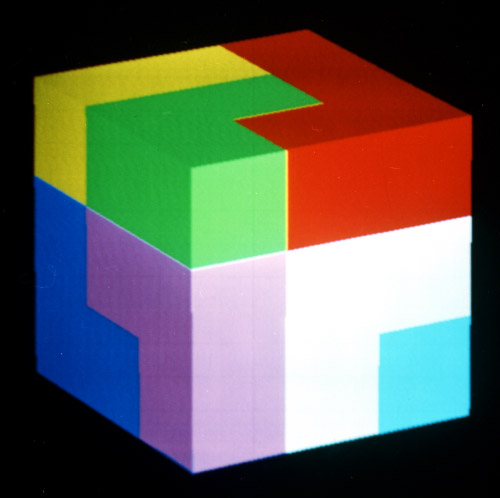
\includegraphics[width=\linewidth]{prviRenderiRomni1.jpg}
			\caption{Рендер склопљене Сома коцке}
		\end{subfigure}
		\begin{subfigure}[b]{0.4\linewidth}
			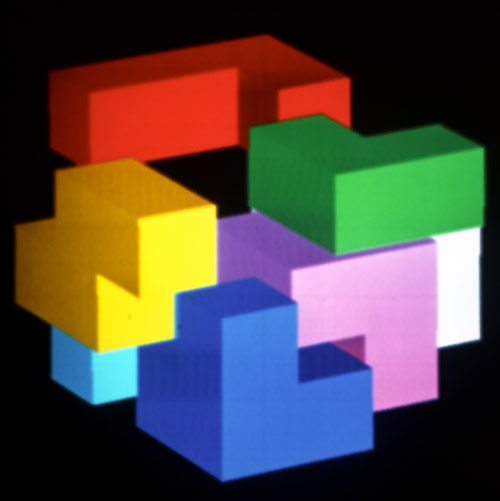
\includegraphics[width=\linewidth]{prviRenderiRomni2.jpg}
			\caption{Рендер раширене Сома коцке}
		\end{subfigure}
		\caption{Рендер сома коцке}
		\label{fig:romni}
	\end{figure}
	
	\begin{figure}[H]
		\centering
		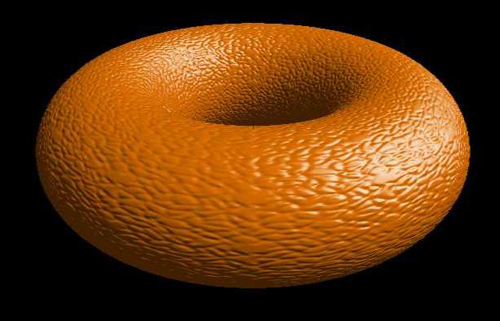
\includegraphics[max width=250pt]{prviRenderiBlin.jpg}
		\caption{Блинов рендер облика торуса}
		\label{fig:blin}
	\end{figure}

	\subsection{Фаза развоја}
	\paragraph{}
	
	\section{Технике рендеровања}
	
	\subsection{Разни алгоритми везани за рендеровање}
	
	\subsubsection{Коен-Сатерландов алгоритам}\label{koensaterland}
	\paragraph{}
	Алгоритам жели да подели екран (гледамо као да је он дводимензионална раван) на 9 једнаких региона и одреди које линије или делови линија припадају средишњем региону. Алгоритам се изводи следећим корацима:
	\begin{enumerate}
		\item Свакој крајњој тачци се припоји код региона. Код региона је четворобитни број који означава у којем се региону налази тачка, први бит је 1 ако се тачка налази изнад средишњег региона, други бит је 1 ако се тачка налази испод средишњег региона, трећи бит је 1 ако се тачка налази десно од средишњег региона, четврти бит је 1 ако се тачка налази лево од средишњег региона.
		\item Линија у целости припада региону ако обе крајње тачке имају код региона 0000.
		\item У супротном, логичка(битска) и операција се врши између кодова региона крајњих тачака.
		\begin{enumerate}
			\item[3.1.] Ако резултат није 0000, линија у целости не припада средишњем региону.
			\item[3.2.] У супротном, морамо да одсечемо део који не припада средишњем региону.
			\begin{enumerate}
				\item[3.2.1.] Изаберемо крајњу тачку линије која не припада средишњем региону.
				\item[3.2.2.] Пронађемо тачку пресека линије са ивицама средишњим регионом која је најближа изабраној крајњој тачци.
				\item[3.2.3.] Изабрану крајњу тачку заменимо са тачком пресека.
				\item[3.2.4.] Поновити корак 2.
			\end{enumerate}
		\end{enumerate}
	\end{enumerate}
	
	\subsubsection{Катмул-Кларков алгоритам}\label{katmulklark}
	\paragraph{}
	Алгоритам жели да дода темена телу тако да се добије облије тело у односу на почетно тело. Пошто овај алгоритам ради на било којем конвексном телу, процес можемо извршити жељени број пута за редом, односно можемо је користити рекурзивно толико пута колико нам је потребно да бисмо добили жељени степен облине.  Алгоритам се изводи следећим корацима:
	\begin{enumerate}
		\item За сваку страну додајемо по једну тачку стране, чију позицију добијамо тиме што узмемо средњу вредност позиција темена које чине ту страну (слика \ref{fig:katmulklark}a).
		\item За сваку ивицу додајемо по једну тачку ивице, чију позицију добијамо тиме што узмемо средњу вредност позиција темена које чине ту ивицу (слика \ref{fig:katmulklark}b).
		\item За свако оригинално теме ($P$) израчунамо средњу вредност ($F$) свих $n$ (које смо мало пре створили) темена страница где страница додирује тачку $P$ и израчунамо средњу вредност ($R$) свих $n$ средишта ивица оригиналних ивица које додирују тачку $P$, где је свако средиште ивица једнако средњој вредности позиција крајева те ивице (слика \ref{fig:katmulklark}c).
		\begin{align}
			P_{novo}&=\frac{F+2R+(n-3)P}{n}
		\end{align}
		
		\item Формирати ивице и стране нове мреже.
		\begin{enumerate}
			\item[4.1.] Повезати сваку нову тачку стране са новим тачкама ивице које припадају оригиналној ивици која је сачињавала оригиналну страну (слика \ref{fig:katmulklark}d).
			\item[4.2.] Повезати нова темена са новим тачкама ивице које припадају оригиналној ивици која је садржала оригинално теме (слика \ref{fig:katmulklark}e).
			\item[4.3.] Оформите нове стране које су затворене новим ивицама (слика \ref{fig:katmulklark}f).
		\end{enumerate}
	\end{enumerate}


	\begin{figure}[H]
		\centering
		\begin{subfigure}{0.3\linewidth}
			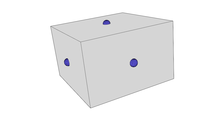
\includegraphics[width=\linewidth]{Catmull-Clark_Recursive_Step_1.png}
			\caption{Тачке стране (плаве сфере)}
		\end{subfigure}
		\begin{subfigure}{0.3\linewidth}
			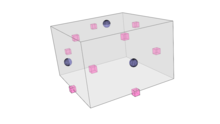
\includegraphics[width=\linewidth]{Catmull-Clark_Recursive_Step_2.png}
			\caption{Тачке ивице (розе коцке)}
		\end{subfigure}
		\begin{subfigure}{0.3\linewidth}
			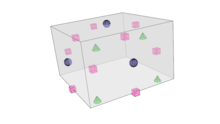
\includegraphics[width=\linewidth]{Catmull-Clark_Recursive_Step_3.png}
			\caption{Нова темена (зелене купе)}
		\end{subfigure}
		\begin{subfigure}{0.3\linewidth}
			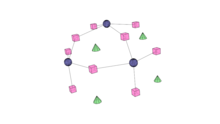
\includegraphics[width=\linewidth]{Catmull-Clark_Recursive_Step_4.png}
			\caption{Нове ивице, четири по тачци стране}
		\end{subfigure}
		\begin{subfigure}{0.3\linewidth}
			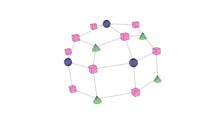
\includegraphics[width=\linewidth]{Catmull-Clark_Recursive_Step_5.png}
			\caption{Три нове ивице по новом темену}
		\end{subfigure}
		\begin{subfigure}{0.3\linewidth}
			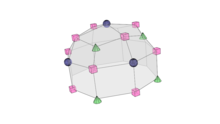
\includegraphics[width=\linewidth]{Catmull-Clark_Recursive_Step_6.png}
			\caption{Завршно додавање страна на мрежу}
		\end{subfigure}
		\caption{Илустрација корака Катмул-Кларковог алгоритма}
		\label{fig:katmulklark}
	\end{figure}
	
	\tableofcontents
	
\end{document}